\documentclass[french, 12pt]{article}

\usepackage{geometry}
 \geometry{
 a4paper,
 total={150mm,240mm},
 left=30mm,
 top=30mm,
 }


\usepackage{helvet}

\usepackage[utf8]{inputenc}
\usepackage[T1]{fontenc}
\usepackage[french]{babel}
\usepackage{comment}
\usepackage{subcaption}
\usepackage{subfiles}
\usepackage{graphicx}
\usepackage[table,xcdraw]{xcolor}
% \usepackage{minted}
\usepackage{placeins}
\graphicspath{ {./img/} }



\title{\fontfamily{phv}\selectfont \Huge \textbf{Panic At Tortuga}}

\author{
    \fontfamily{phv}\selectfont
    \vspace{15pt}
    Harrys KEDJNANE\\
    % \texttt{harrys.kedjnane@epita.fr}
    % \and
    \vspace{15pt}
    \fontfamily{phv}\selectfont
    Renaud-Dov DEVERS\\
    % \texttt{renaud-dov.devers@epita.fr}
    % \and
    \vspace{15pt}
    \fontfamily{phv}\selectfont
    Julien COHEN-SCALI\\
    % \texttt{julien.cohen-scali@epita.fr}
    % \and
    \fontfamily{phv}\selectfont
    Paul DE LA PORTE DES VAUX\\
    % \texttt{paul.de-la-porte-des-vaux@epita.fr}
    
}
\date{\fontfamily{phv}\selectfont Janvier 2021}

\begin{document}

\begin{titlepage}
    \maketitle
    \thispagestyle{empty}
    % {\fontencoding{T1}\fontfamily{calligra}\selectfont the font is temporarily changed}
    \vspace{20pt}
    \begin{figure}[hbt!]
        \centering
        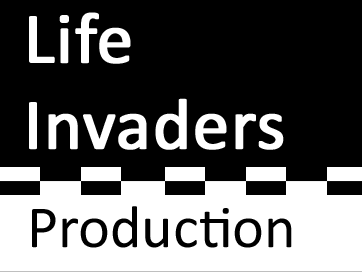
\includegraphics[scale=0.7]{logo_lifeinvaders_copie.png}
    \end{figure}
\end{titlepage}

\begin{center}
    \textbf{Introduction}

    Nous allons vous présenter notre projet de S2.
    Notre équipe a choisi de réaliser un jeu vidéo pour le projet de l'Info SUP.
\end{center}

\tableofcontents
\newpage

\section{Introduction}
\subsection{Présentation du jeu}
\begin{flushleft}
    Panic At Tortuga est un jeu multijoueur dans lequel les différents joueurs doivent s'entre-éliminer sur une île.
    Le jeu s'inspire de jeux connus : Le premier est le mod "Guess Who ?"\footnote{Lui même inspiré de jeux tels que Hide \& Seek, Spy Party ou encore Prop Hunt} de Garry's Mod
        où une première équipe doit rechercher et éliminer l'autre équipe qui s'est déguisée en NPC (Non-Player Character) et qui doit imiter les mouvements aléatoires du bot.
    Le deuxième jeu dont nous nous sommes inspirés est le mode multijoueur proposé dans quelques jeux Assasin's Creed.
    Dans ce mode, chacun des joueurs se voit attribuer une cible, ce qui fait que tous les joueurs sont à la fois des traqueurs et traqués.

    Notre jeu se passera sur une île tropicale fictive dans les Caraïbes.
    L'objectif est de se cacher parmi la foule d'une petite île perdue au beau milieu de l'océan et d'éliminer votre cible sans être vu.
\end{flushleft}

\subsection{L'équipe de LifeInvaders}
\textbf{DEVERS Renaud-Dov (Chef de Projet)} \\
J'adore l'informatique depuis des années, je suis tombé dans la marmite des vieux ordinateurs (Windows 2000 !) à disquette quand j'était petit.

J'aime les travaux et les projets de groupe, en ayant trois à mon actif, dont le projet d'ISN et celui de SI. J'ai pu réaliser par exemple une application dynamique pour libraires avec une connexion à la database de Google Books.
J'y ai appris le rôle d'un chef de groupe, de l'organisation à la responsabilité, je trouve les projets formateurs.
Ce projet sera donc l'occasion de m'améliorer dans le travail de groupe, pour être prêt pour le monde professionnel.
\newline
\textbf{KEDJNANE Harrys} \\
Avant EPITA, je faisais une PACES et je n’avais jamais codé 
même si l’informatique est un sujet qui m’a toujours fortement intéressé. 
Depuis mon arrivé à cette école, j’ai découvert les joies de la programmation 
et ce projet me permettra d’approfondir ce sujet appliqué à un autre milieu 
qui m’intéresse tout autant: le jeu vidéo. 
\newline
\textbf{DE LA PORTE DES VAUX Paul} \\
Ayant découvert le monde de l’informatique assez tard, je n’ai fait que des petits projets, comme des Hackintosh ou des projets python de cryptographie et de reconnaissance d’objets.
La création d’un jeu en 3D m’enchante donc, car elle va me permettre d’explorer de nouveaux horizons.
\newline
\textbf{COHEN-SCALI Julien} \\
Étant un gros joueur et passionné depuis mon enfance, ce projet est un moyen pour moi de m’exprimer grâce aux différents cours de programmation en C\#.
Par ailleurs, ayant fait un stage à l’ISART, le C\# et Unity ne me sont pas inconnus. De plus, ce projet est un bon moyen de s’exercer à la Programmation Orientée Objet vue lors derniers cours de programmation,
ce qui permettra à notre groupe d’améliorer notre code et d’acquérir une méthode bien plus professionnelle, nous préparant à notre vie future.
La collaboration autour du projet et l’importance de travailler en groupe grâce a git développe en chacun de nous un esprit d’équipe conséquent.
Ce projet est donc, pour moi, un très bon entrainement pour le développement de projet dans ma vie futur. (mais aussi un très bon moyen de s’amuser).

\subsection{Identité visuelle}
Pour créer le logo de notre jeu, nous avons utilisé Photoshop pour faire un logo stylisé, dans les mêmes tons que propose notre jeu.
\begin{figure}[hbt!]
    \centering
    
\includegraphics[scale=0.5]{logo.png}
    \caption{Logo de Panic At Tortuga}
\end{figure}

\section{Choix techniques}

Nous avons décidé de réaliser un jeu en 3D sur le moteur cross-platform de Unity Technologies.
Ce moteur est complet et possède plein de fonctionnalités pour créer un environnement jeu fonctionnel.

Nous avons décidé d'acheter un asset contenant de multiples textures, prefabs, objets et personnages sur le thème des pirates et des Caraïbes.\footnote{Voir Partie Coûts de production}
Nous n'aurons donc pas, sauf quelques rares modèles, besoin de modéliser des mesh sur Blender.

Nous avons choisi d'intégrer l'outil PUN 2 de Photon pour la réalisation du multijoueur et l'interaction entre joueurs.


\newpage
\section{Répartition des tâches}

\begin{table}[!htb]
    \begin{tabular}{|l|l|l|}
    \hline
    \textbf{Tâche}                         & \textbf{Responsable}               & \textbf{Suppléant}                 \\ \hline
    \multicolumn{3}{|l|}{\cellcolor[HTML]{343434}{\color[HTML]{FFFFFF} \textbf{Carte}}}                              \\ \hline
    Création de la carte                   & \cellcolor[HTML]{9698ED}Paul       & \cellcolor[HTML]{34FF34}Renaud-Dov \\ \hline
    Création du lobby                      & \cellcolor[HTML]{34FF34}Renaud-Dov & \cellcolor[HTML]{9698ED}Paul       \\ \hline
    \multicolumn{3}{|l|}{\cellcolor[HTML]{343434}{\color[HTML]{FFFFFF} \textbf{Réseau}}}                             \\ \hline
    Implémentation du multijoueur          & \cellcolor[HTML]{34CDF9}Julien     & \cellcolor[HTML]{F8A102}Harrys     \\ \hline
    \multicolumn{3}{|l|}{\cellcolor[HTML]{343434}{\color[HTML]{FFFFFF} \textbf{IA}}}                                 \\ \hline
    Réalisation des différents types d'IA  & \cellcolor[HTML]{34FF34}Renaud-Dov & \cellcolor[HTML]{9698ED}Paul       \\ \hline
    \multicolumn{3}{|l|}{\cellcolor[HTML]{343434}{\color[HTML]{FFFFFF} \textbf{Menus}}}                              \\ \hline
    Interface                              & \cellcolor[HTML]{34CDF9}Julien     & \cellcolor[HTML]{F8A102}Harrys     \\ \hline
    HUD                                    & \cellcolor[HTML]{F8A102}Harrys     & \cellcolor[HTML]{34CDF9}Julien     \\ \hline
    \multicolumn{3}{|l|}{\cellcolor[HTML]{343434}{\color[HTML]{FFFFFF} \textbf{Game Core}}}                          \\ \hline
    Contrôle du personnage                 & \cellcolor[HTML]{34FF34}Renaud-Dov & \cellcolor[HTML]{F8A102}Harrys     \\ \hline
    Animations                             & \cellcolor[HTML]{34FF34}Renaud-Dov &                                    \\ \hline
    Objets dynamiques                      & \cellcolor[HTML]{34FF34}Renaud-Dov & \cellcolor[HTML]{F8A102}Harrys     \\ \hline
    Déroulé d'une partie                   & \cellcolor[HTML]{F8A102}Harrys     & \cellcolor[HTML]{9698ED}Paul       \\ \hline
    \multicolumn{3}{|l|}{\cellcolor[HTML]{343434}{\color[HTML]{FFFFFF} \textbf{Autre}}}                              \\ \hline
    Système de progression                 & \cellcolor[HTML]{F8A102}Harrys     &                                    \\ \hline
    Réalisation et maintenance du site Web & \cellcolor[HTML]{9698ED}Paul       & \multicolumn{1}{c|}{-}             \\ \hline
    \end{tabular}
    \end{table}

\newpage
\subfile{sections/mouvements.tex}
\newpage
\subfile{sections/gameplay.tex}
% \newpage
\subfile{sections/organisation.tex}
\newpage
\subfile{sections/progression.tex}
\subfile{sections/hud.tex}
% \newpage
\subfile{sections/ai.tex}
\newpage
\subfile{sections/multiplayer.tex}
\newpage
\subfile{sections/map.tex}
\newpage
\subfile{sections/costs.tex}
\section{Autres liens utiles}
\end{document}